\documentclass{article}

\usepackage{graphicx}
\usepackage{physics}
\usepackage{subcaption}
\usepackage{hyperref}
\usepackage{float}

\usepackage[left=2.5cm, right=2.5cm, top=2cm, bottom=2cm]{geometry}
\setlength{\parindent}{0em}
\setlength{\parskip}{0.8em}

\usepackage{caption}
\captionsetup{width=.9\textwidth}

\usepackage{biblatex}
\addbibresource{report.bib}

\title{Exercise 2, TFY4235 Computational physics}
\author{Martin Johnsrud}
\vspace{-8ex}
\date{}


\begin{document}
    \maketitle
    \section*{Introduction}
    This report documents the simulation of magnons, as described in \cite{exercise}.
    Using Heun's method, the Landau-Lifshitz-Gilbert equations for a classical, interacting ensemble of spins are integrated in time.
    The algorithm is first used to simulate one spin, for which the exact solution is known.
    Then, the formation of collective modes, magnons, are simulated, and difference between ferromagnetic and anti-ferromagnetic materials and magnetization is investigated.

    \section*{Theory}
    \subsection*{Units}

    The Hamiltonian and the equations of motion as given in \cite{exercise} gives natural units for this problem,
    \begin{itemize}
        \item Energy: $[\mathcal H] = [J]$
        \item Magnetic field and magnetization: $[\vec B] = [\vec M] = [\vec S /\mu ]$
        \item Anisotropy: $[d_z] = [J]$
        \item Time : $[t] = [\mu/\gamma J]$
    \end{itemize}
    The dynamical variables of the problem, $ \vec S $, are assumed to be dimensionless, and normalized to $|\vec S|\in[0, 1]$.
     The defining dimensionful constants of the system are thus the coupling $J$, the magnetic moment $\mu$ and the gyromagnetic ratio $\gamma$.
     These units are used throughout the exercise, including in all figures.
     Physical values for a given, actual system is then dependent on its values for $J, \mu$ and $\gamma$, as well as substitution $\vec S \rightarrow S_0 \vec S$, where $S_0$ is the physical magnitude of the spins.
     In this paper as well as in the code it documents, all equations and quantities are given in these units, including the Hamiltonian \autoref{hamiltonian}, and the equations of motion \autoref{LLG} and \autoref{effective field}.


    \subsection*{Indices}
    For easy implementation, the Hamiltonian can be written on index form and using the units as described above
    \begin{equation}
        \mathcal{H}(S; J, d_z, B) = -\frac{1}{2} J \sum_{\langle i, j \rangle, a} S_{i, a} S_{j, a} - d_z \sum_{j} (S_{j,3})^2 -  \sum_{j, a} B_{j, a} S_{j,a}.
        \label{hamiltonian}
    \end{equation}
    Here, $J\in\{-1, 0, 1\}$, $i\in\{1, ..., N\}$ is the site index, $a$ is vector component index.
    The effective field can be written
    \begin{align*}
        H_{k, b} = - \pdv{\mathcal{H}}{S_{k, b}} = \frac{1}{2} J \sum_{\langle i, j \rangle, a} (S_{i, a}\delta_{j,k}\delta_{a, b} + S_{j, a}\delta_{i,k}\delta_{a, b}) + 2 d_z \sum_{j} S_{j,3} \delta_{b, 3}\delta_{j, k} +  \sum_{j, a} B_{j, a} \delta_{k,b},
    \end{align*}
    using the vector triple product identity $\vec A \times (\vec B \times \vec C) = (\vec A \cdot \vec B) \vec C - (\vec A \cdot \vec C) \vec B$.
    The first sum becomes
    \begin{equation*}
        \frac{1}{2}\sum_{\langle i, j \rangle, a} (S_{i, a}\delta_{j,k}\delta_{a, b} + S_{j, a}\delta_{i,k}\delta_{a, b}) = \frac{1}{2}\sum_{\langle i, j \rangle} (S_{i, b}\delta_{j,k} + S_{j, b}\delta_{i,k}) = \frac{1}{2}\sum_{\langle j, i \rangle} 2S_{i, b} \delta_{j, k} = \sum_{j \in \mathrm{NN}_k} S_{j, b},
    \end{equation*}
    where $\mathrm{NN}_k$ are the set of nearest neighbours of lattice point $k$.
    The Landau-Lifshitz-Gilbert equation for the time evolution of the system is then
    \begin{align}
        \dv{t} S_{j, a} &= - \frac{1}{(1 + \alpha^2)}\left[\sum_{b c}\varepsilon_{abc}S_{j, b}H_{j,c} + \alpha \sum_{b}\left(S_{j, b}S_{j, b}H_{j, a} - S_{j, b}H_{j, b}S_{j, a}\right)\right], \label{LLG} \\
        H_{k, b} &= J\sum_{j \in \mathrm{NN}_k} S_{j, b} + 2d_z S_{k, 3} \delta_{k, 3} +  B_{k, b}.
        \label{effective field}
    \end{align}

    
    \section*{Implementation}
    The main object of the simulation is a NumPy-array \verb|S| of shape \verb|(T, N, 3)|.
    This contains the components of each of the $N$ spins at each time step.
    The function \verb|integrate| then runs a loop, calling the implementation of Heun's method \verb|heun_step|.
    The index notation laid out in the Theory section allows for straight forward implementation of the LLG equation using NumPy's \verb|einsum|-function.
    For example, using a array \verb|eijk[a, b, c]| for the Levi-Civita symbol, 
    $$
    \sum_{b c}\varepsilon_{abc}S_{j, b}H_{j,c}
    $$
    becomes
    \begin{center}
        \verb|np.einsum("...ac, ...c-> ...a", np.einsum("abc, ...b -> ...ac", eijk, S), H)|.

    \end{center}

    \verb|LLG| takes as arguments \verb|S| and the needed parameters.

    Then, it first evaluates the first sum of \autoref{LLG} as shown above.
    If $\alpha \neq 0$, it then evaluates the second sum.
    \verb|LLG| calls \verb|get_H|.
    This functions implements \autoref{effective field}, using NumPy's \verb|roll|-function to sum over all nearest neighbours.
    This automatically implements periodic boundary conditions.
    \verb|LLG| then returns \verb|dtS|, a NumPy-array containing the time derivative of $S$.
    This implementation makes it easy to generalize to spins distributed in 2 or 3 dimensions, as is done in \verb|3D.py|.
    The only change needed is to extend the shape of \verb|S| to \verb|(T, N, N, N, 3)|, and change \verb|get_H| to sum over nearest neighbours in all dimensions.

    The library \verb|mayavi| is used to make 3D visualization of the spins, as in \autoref{ground states 3D} and to make videos of the time evolution of the spins.
    \verb|ffmpeg| is then used to use the snapshots from \verb|mayavi| to make a video.
    Videos of one spin, a chain of spins and a configuration of spins in 3D is included in the folder \verb|plots|.


    \section*{Results}
    \subsection*{Single spin}

    The first test of the simulation is to initialize a single spin, in a magnetic field $B = (0, 0, 1)$.
    This spin is given a slight tilt, with initial conditions $(\theta, \phi) = (0.5, 0)$.
    As the torque on the spin is 
    \begin{equation*}
        \vec \tau = \dv{\vec S}{t} = \vec{S} \times \vec{B},
    \end{equation*}
    the expectation is that the spin will precess in a circle around the $z$-axis, with a Larmor frequency $\omega = -B$.
    \autoref{single spin} shows the $x,y$-components of this spin as a function time, together with the expected analytical result.
    The video \verb|plots/test.mp4| shows a animation of the motion of an arrow representing the spin. On the right, the plot shows the error in each components.
    The error in the $z$ component can then be tested checking the deviation from $\vec S^2=1$, which in this case was around $10^{-7}$.

    To analyze the convergence of the method, the simulation is run with different step lengths $h$, for the same simulation time $t_0 = 5$.
    The result is shown in \autoref{error}.
    As Heun's method is of higher order than Euler's method, it converges faster.
    It is, however, necessary to make 2 function calls when using Heun's method, while Euler's method only require one.
    This should make Euler's method twice as fast, which was observed.
    Euler's method ran at around 16\,000 iterations per second, while Heun's method only ran at 8\,000.
    The large gain in precision, however, makes Heun's method preferred for this application. 
    Throughout this exercise, the step length used is $h=0.01$, as it is deemed to give high enough precession.

    \begin{figure}[H]
        \begin{subfigure}{.49\textwidth}
            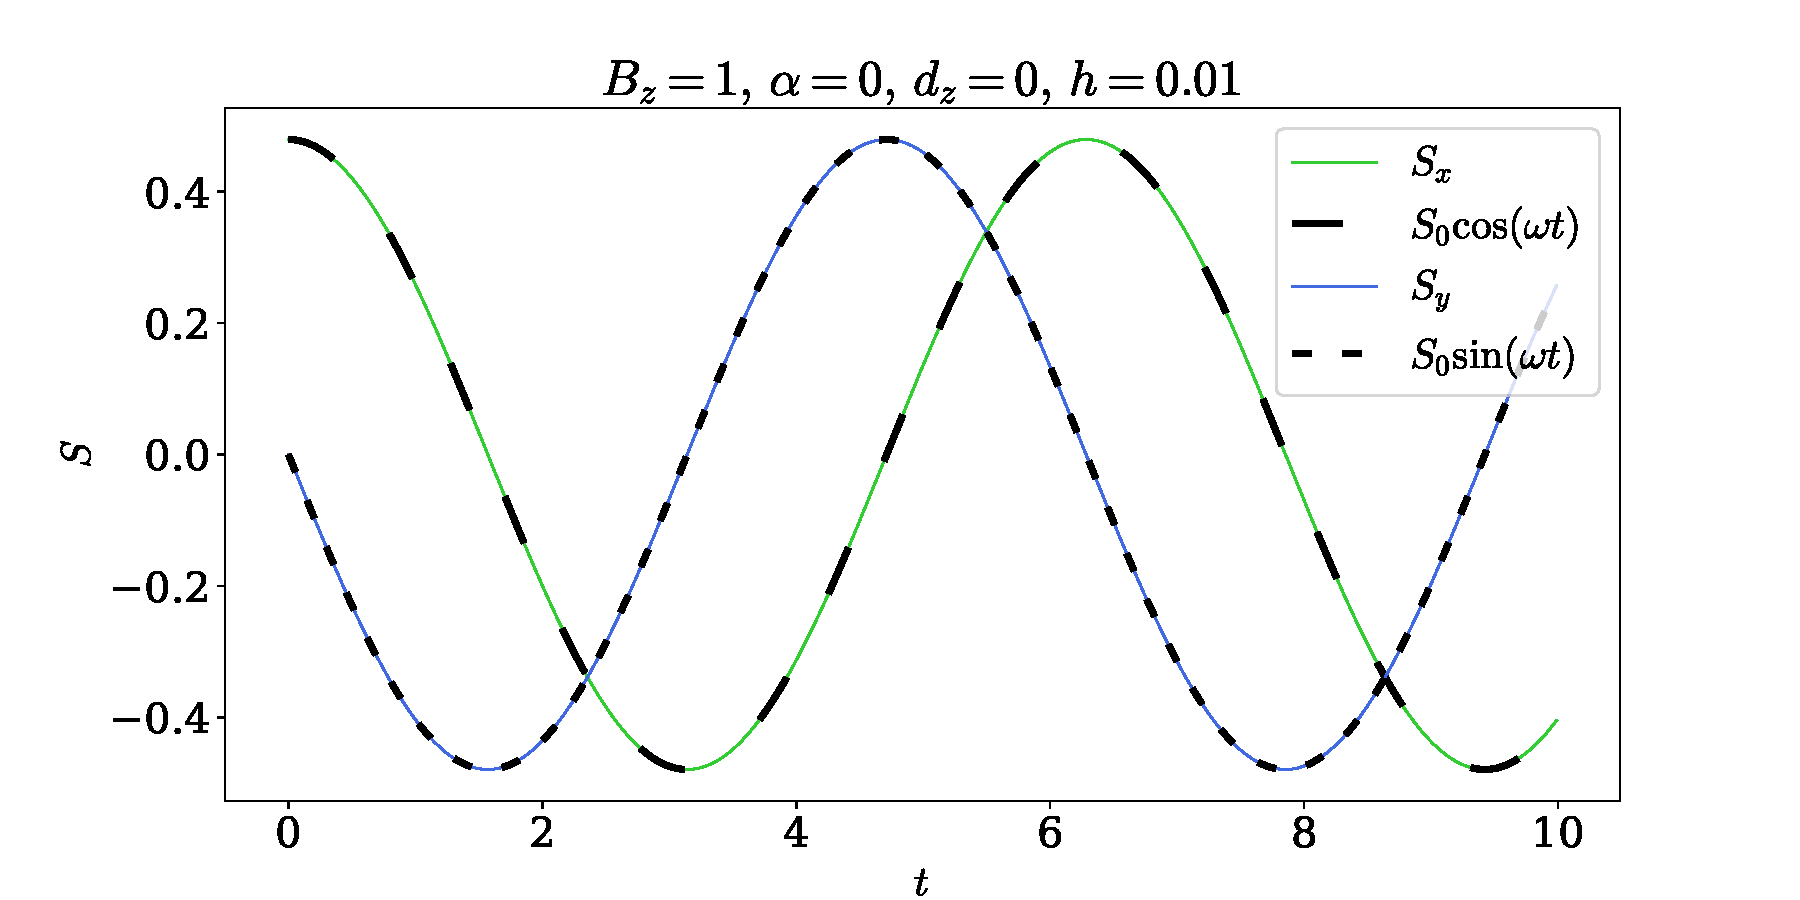
\includegraphics[width=1.1\textwidth]{../plots/single.pdf}            
        \end{subfigure}
        \begin{subfigure}{.49\textwidth}
            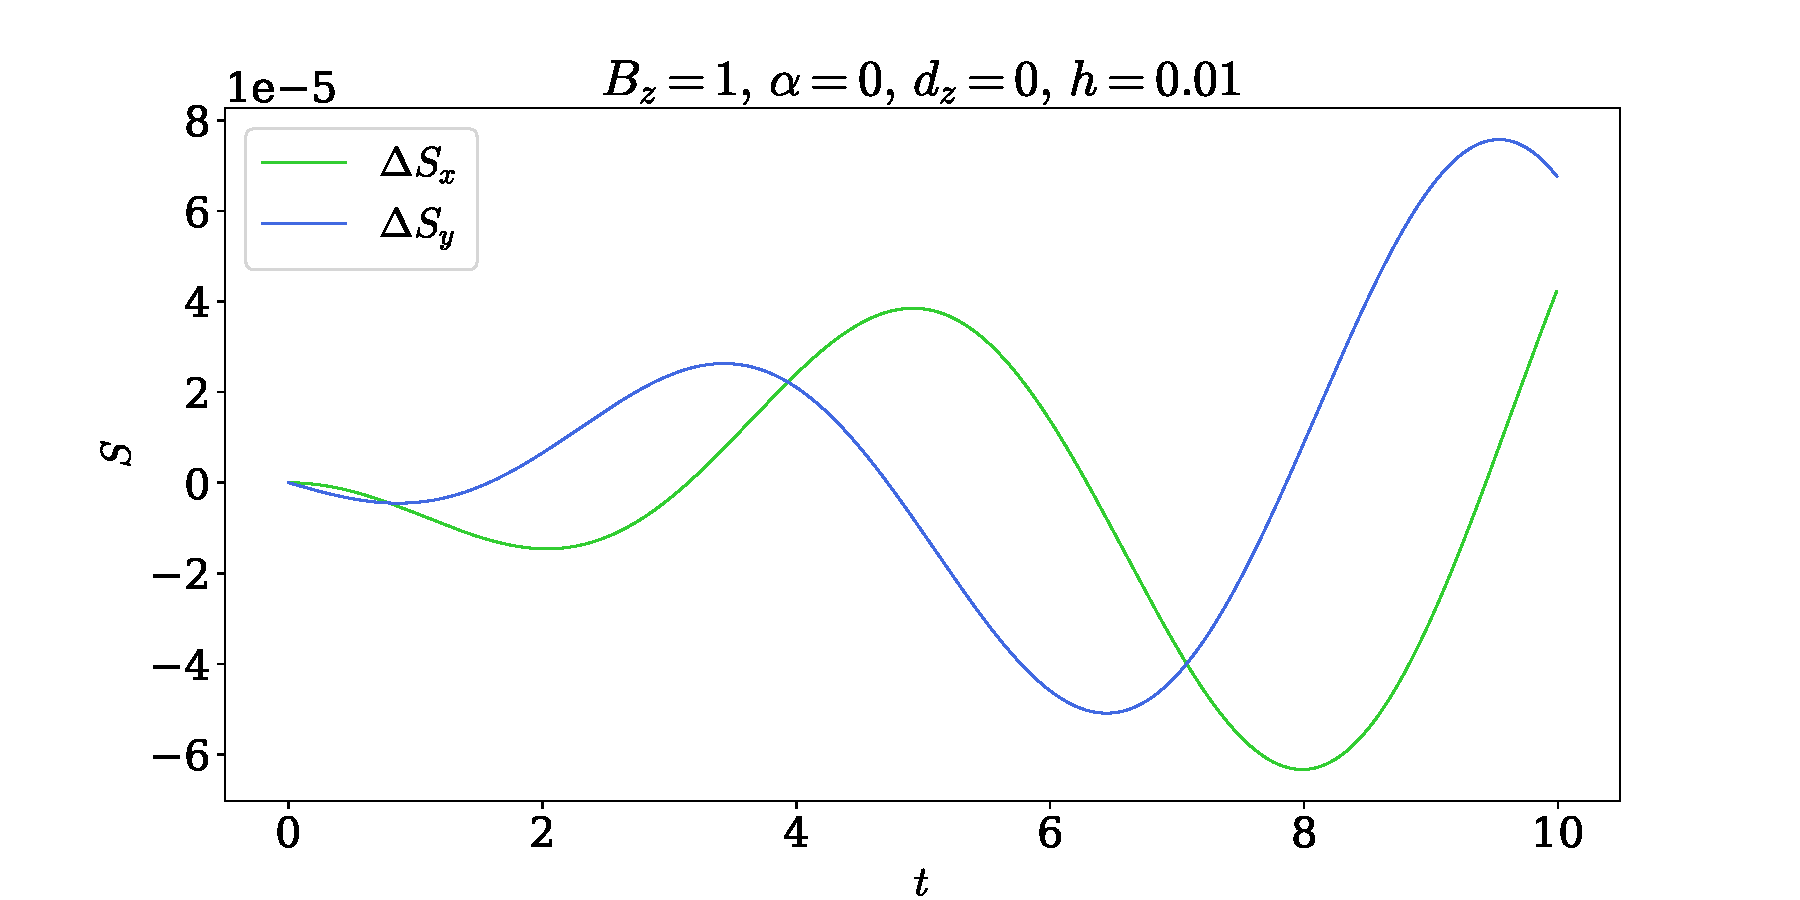
\includegraphics[width=1.1\textwidth]{../plots/single_diff.pdf}            
        \end{subfigure}
        \caption{On the left, motion of the $x$ and $y$ component of the spin in a constant magnetic field, together with the analytical result. On the right, the difference between the simulated and the analytical result.}
        \label{single spin}
    \end{figure}

    \begin{figure}[H]
        \centering
        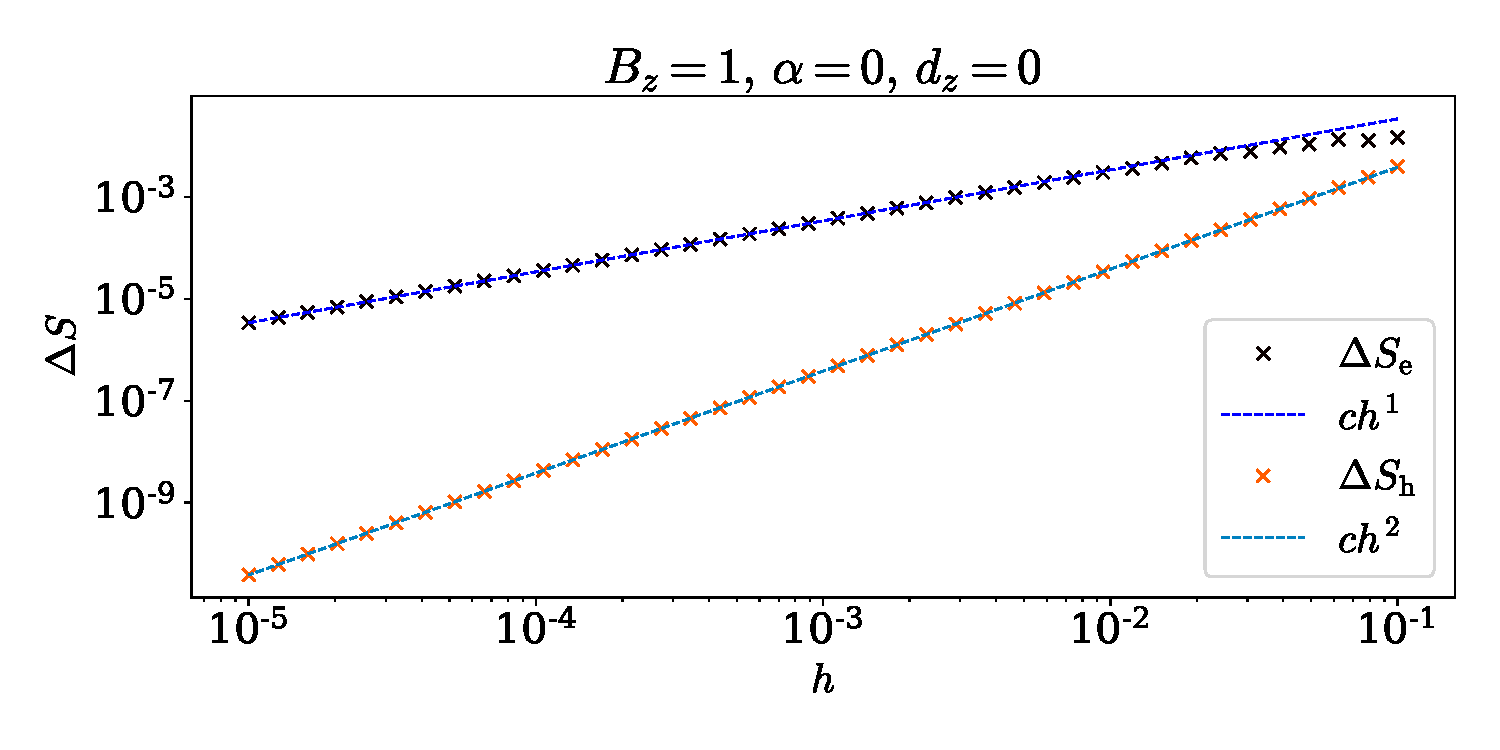
\includegraphics[width=.7\textwidth]{../plots/err.pdf}
        \caption{The error from the simulation using the euler method, $\Delta S_e$ and Heun's method, $\Delta S_h$.}
        \label{error}
    \end{figure}

    When including $\alpha > 0$, one should expect the the oscillations to die away, with a lifetime given by
    \begin{equation*}
        \tau = \frac{1}{\alpha \omega}.
    \end{equation*}
    Larger $\alpha$ should give a shorter lifetimes, and thus faster decay.
    \autoref{decay} shows this.
    Furthermore, we see that the amplitude is proportional to $\exp(-t/\tau)$.
    We should expect this, not only is this a common form for decay, but as no time is special, the decay should be proportional to the amplitude, which gives exponential decay.

    \begin{figure}[H]
        \centering
        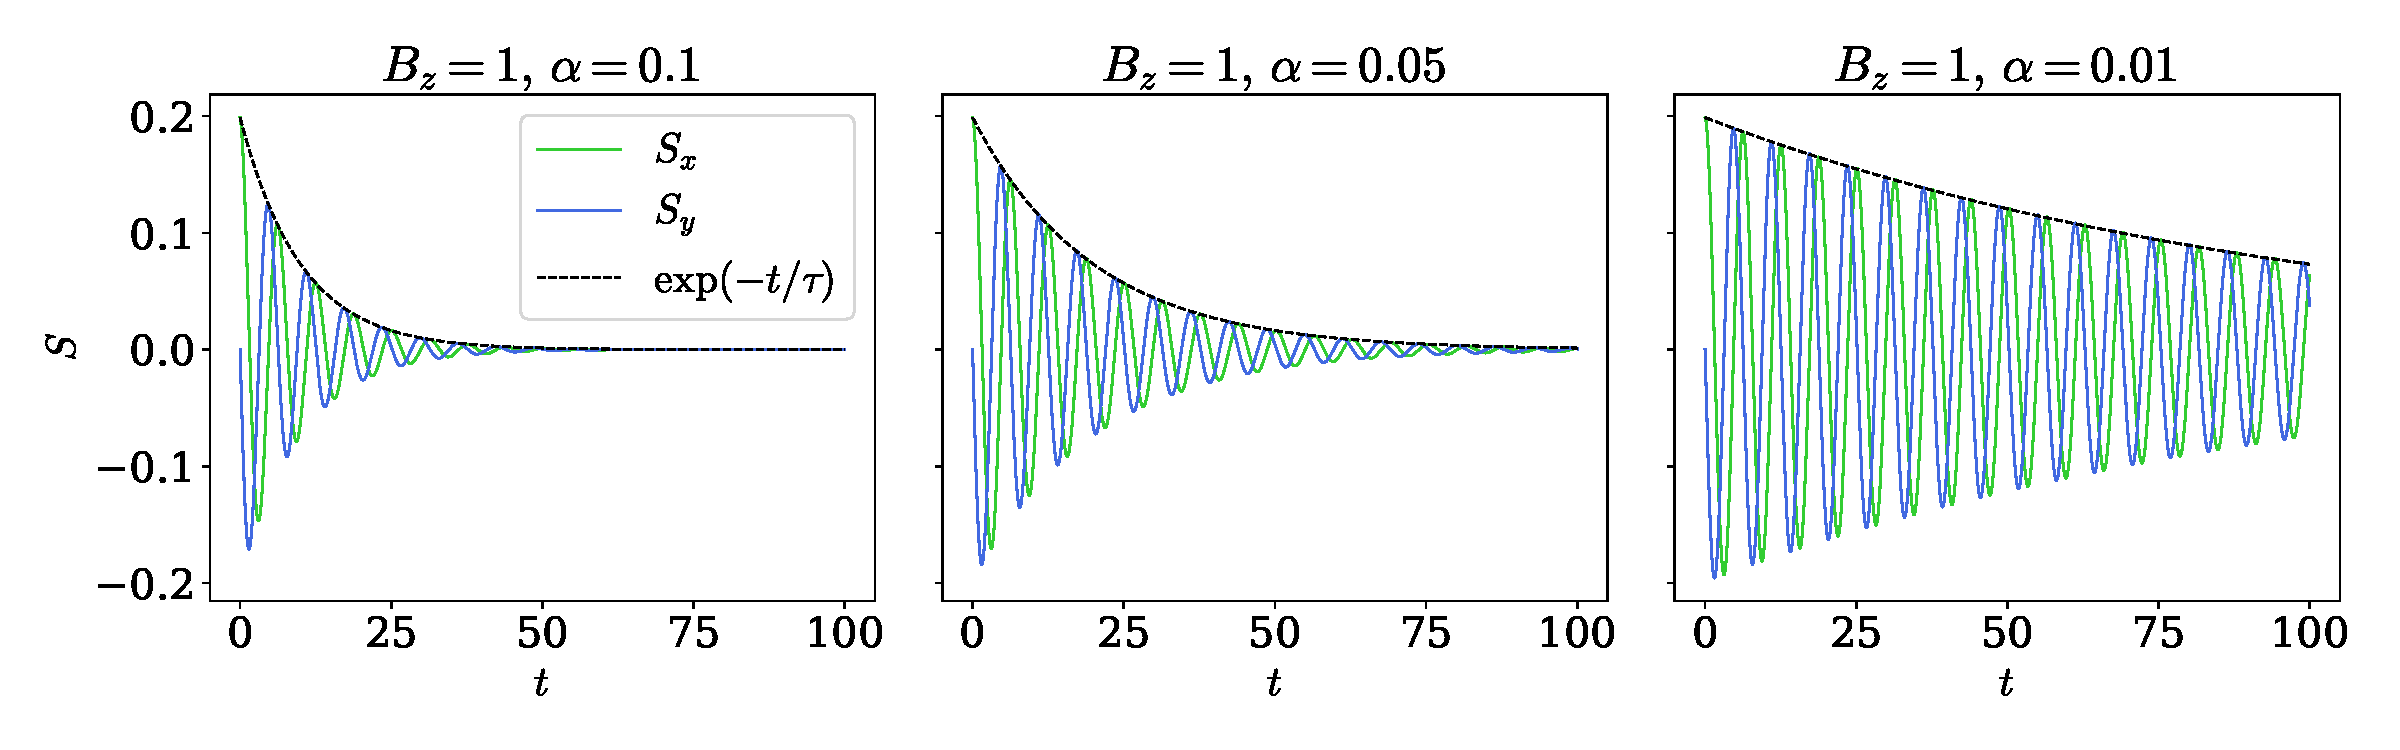
\includegraphics[width=\textwidth]{../plots/decay_a.pdf}
        \caption{The decay of the oscillation of a single spin, for different values of $\alpha$.}
        \label{decay}
    \end{figure}

    \subsection*{Spin chain}
    The simulation now includes several spins, in a ferromagnetic or anti-ferromagnetic coupling, depending on if $J = 1$ or $J = -1$, respectively.
    When including damping $\alpha > 0$, both these settle into the ground state of the system, after some time.
    This is shown in \autoref{ground states}.
    However, the two systems have different ground states.
    In the ferromagnetic case, the lowest energy configuration is the alignment of all the spins, while in the anti-ferromagnetic case the spins are oppositely aligned.
    The final configurations of both systems are shown in \autoref{ground states 3D}.

    \begin{figure}[H]
        \centering
        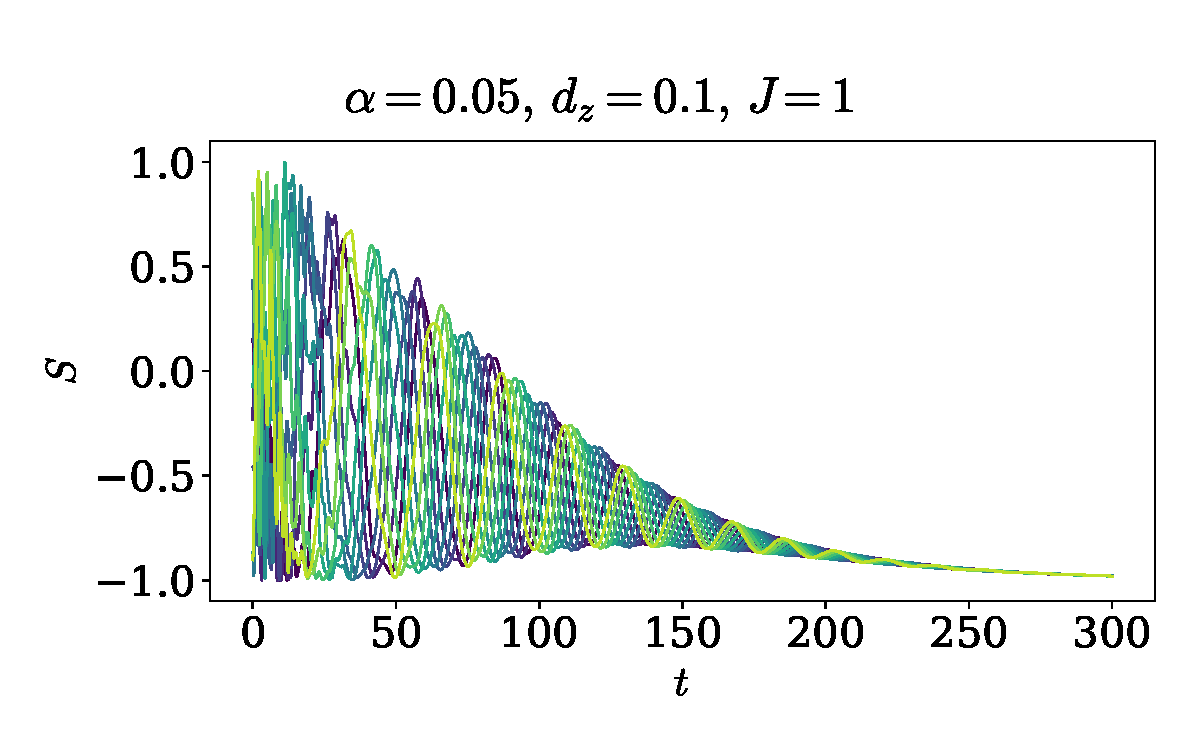
\includegraphics[width=0.49\textwidth]{../plots/ground_state_f.pdf}
        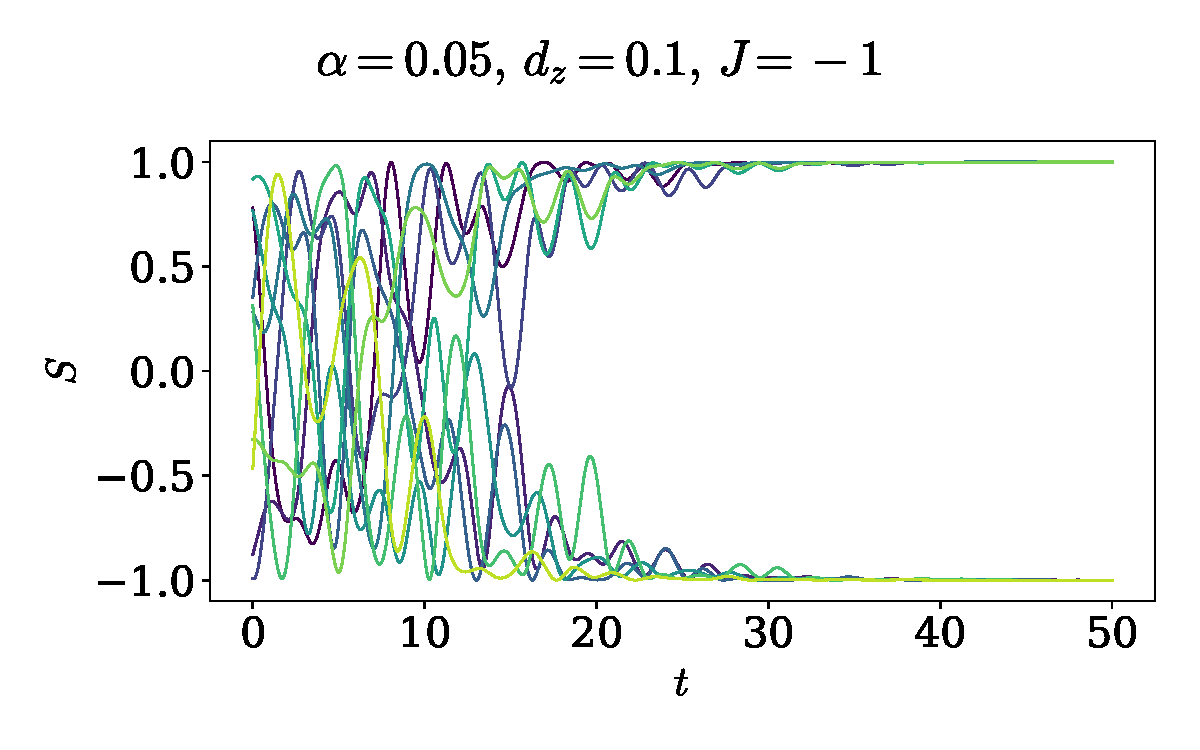
\includegraphics[width=0.49\textwidth]{../plots/ground_state_af.pdf}
        \caption{The $z$-component of all the spins in a ferromagnetic (left) and anti-ferromagnetic(right) spin chain. As $\alpha>0$, the states settle down into theri ground state.}
        \label{ground states}
    \end{figure}
    \begin{figure}[H]
        \centering
        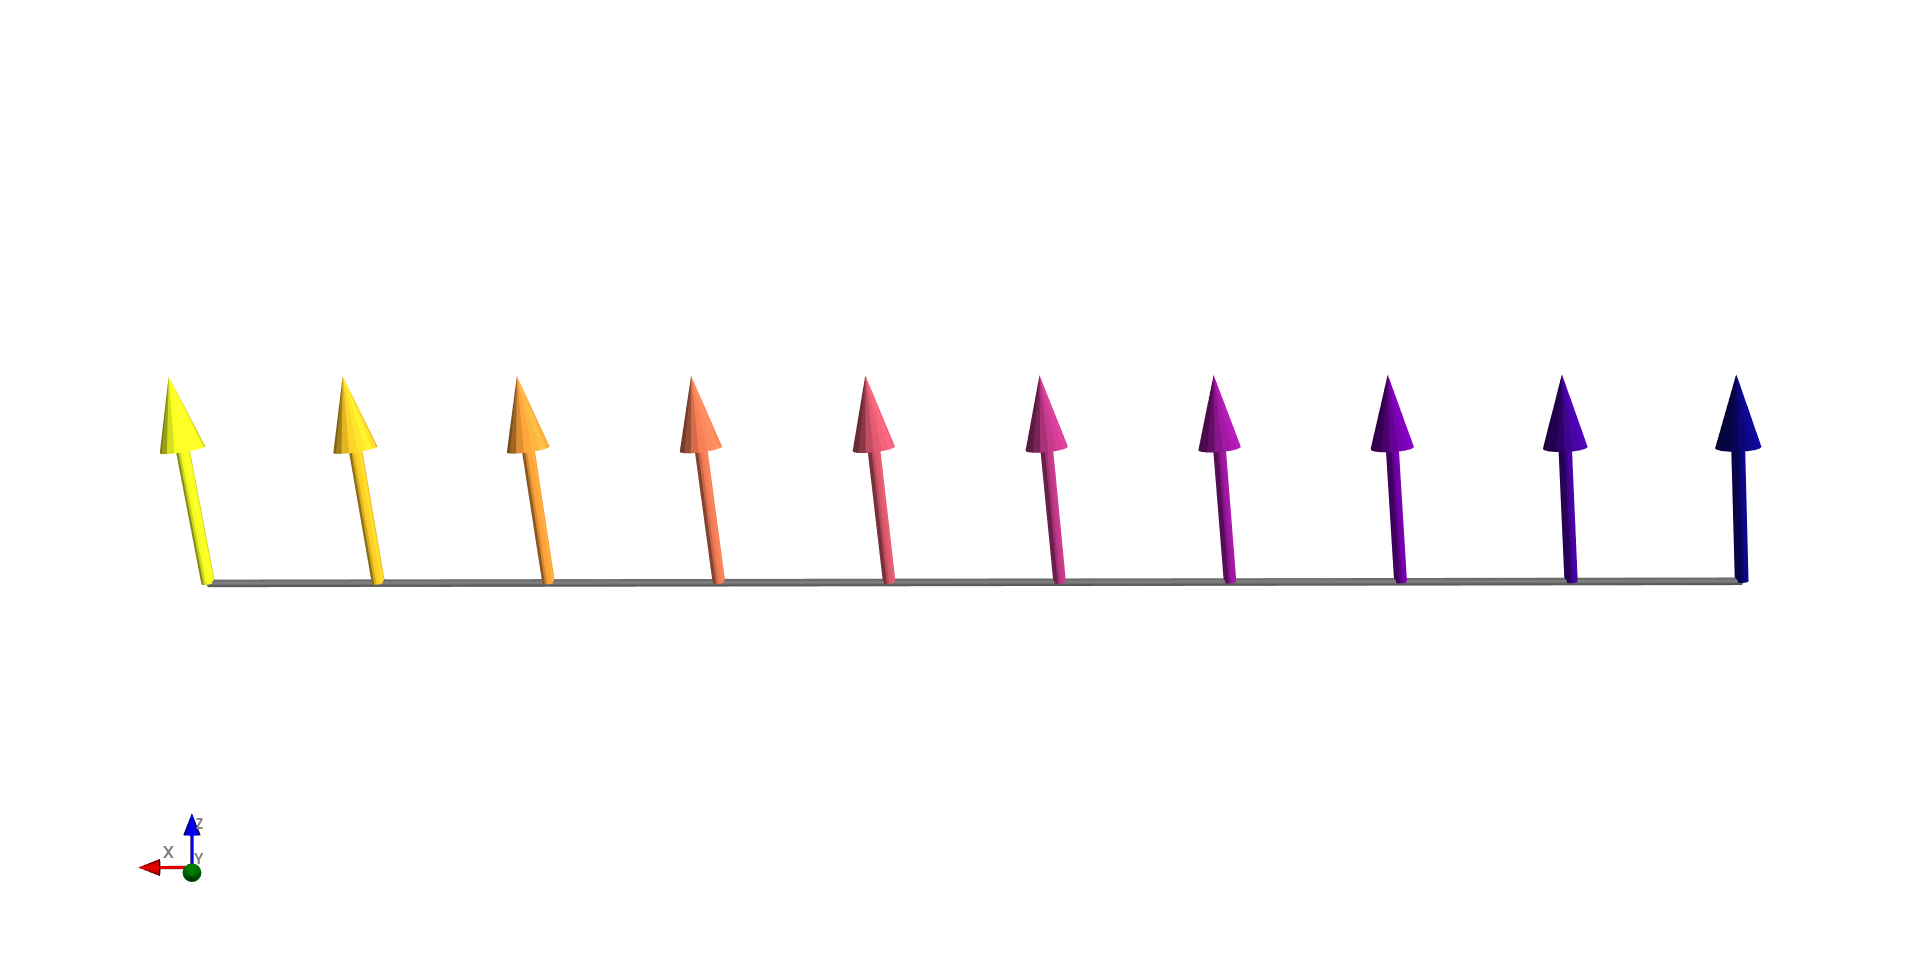
\includegraphics[width=0.49\textwidth]{../plots/ground_state_f3D.png}
        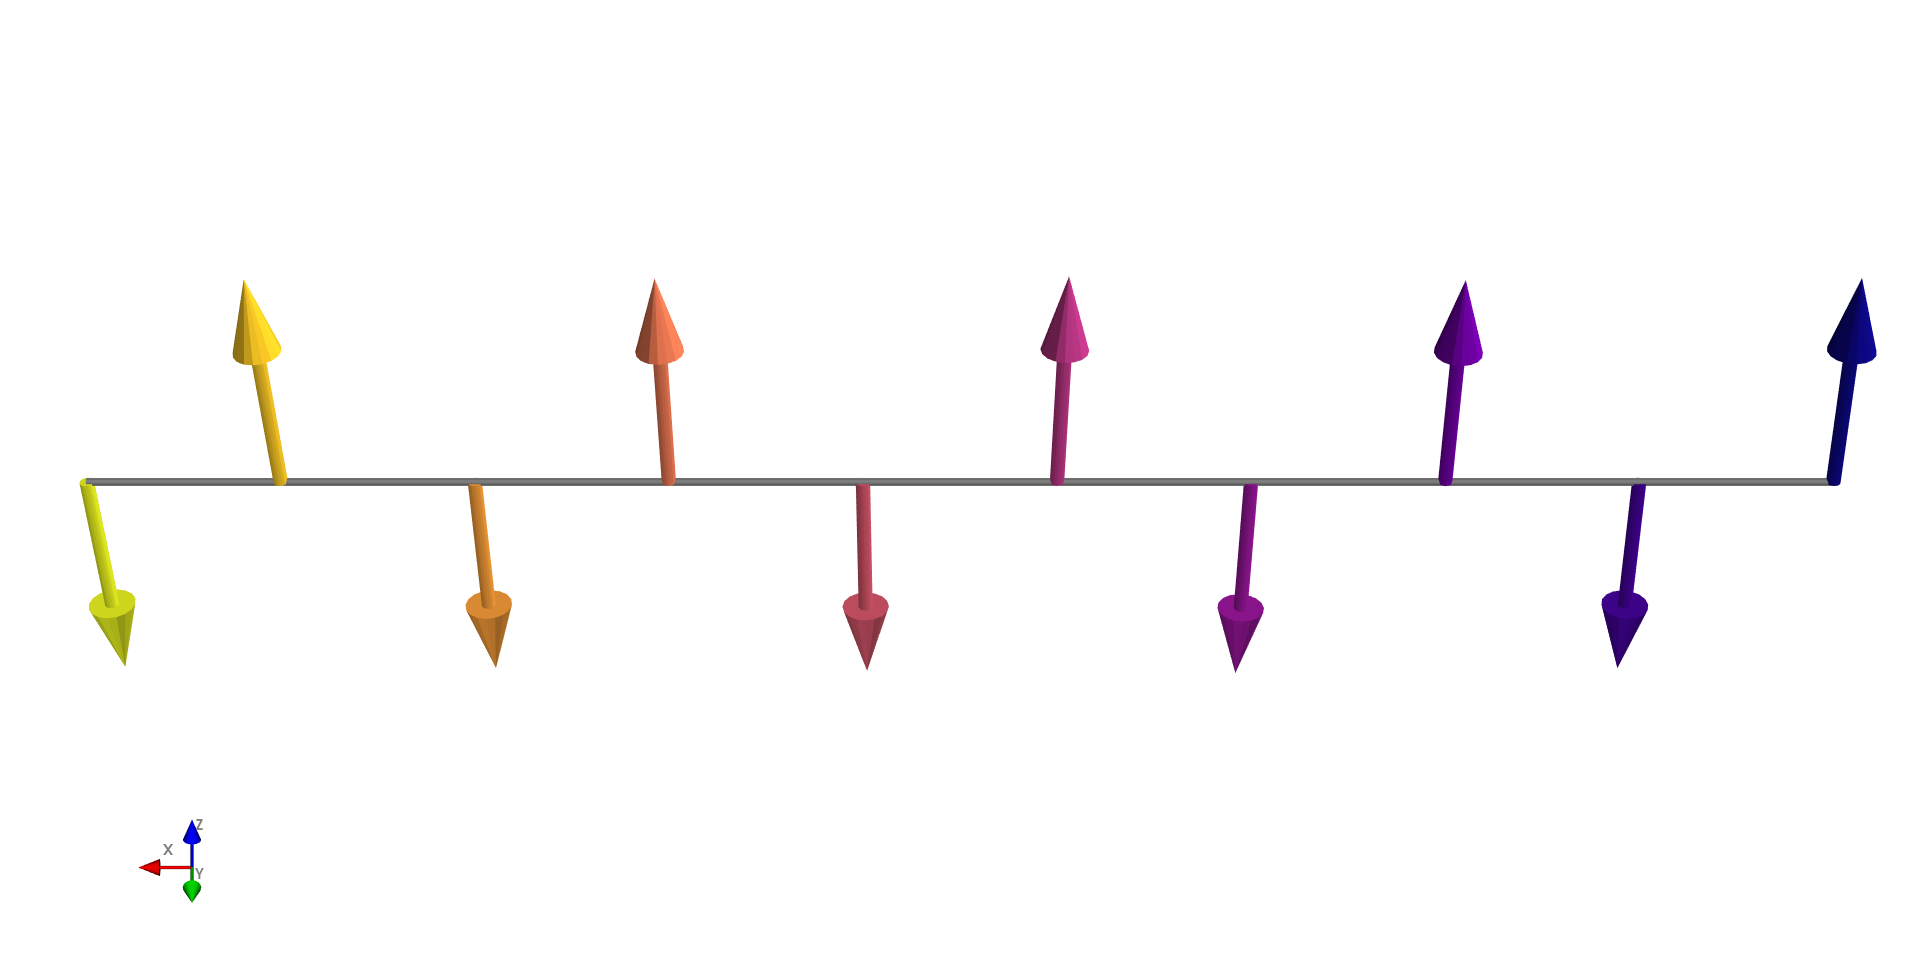
\includegraphics[width=0.49\textwidth]{../plots/ground_state_af3D.png}
        \caption{The ground state of ferromagnetic (left) and anti-ferromagnetic (right) spin chains.}
        \label{ground states 3D}
    \end{figure}

    When the coupling is turned of, $J = 0$, but $d_z>0$ and the spins are initialized randomly, they will all precess around the $x$-axis, with different frequencies, as shown in \autoref{all tilted}.
    This is because it is now an uncoupled system, where each spin follows 
    \begin{equation*}
        \dv{\vec S}{t} = - 2 d_z S_z \,\vec S \times \hat z, 
    \end{equation*}
    i.e.
    circular precession around the $z$-axis.
    Thus, spins parallel to the $z$-axis should not move, while the one tilted spin precesses.
    If only one spin is tilted, it will precess alone, as shown in to the left in \autoref{one tilted}.
    However, if the coupling is turned on again, as shown on the right in \autoref{one tilted}, the disturbance will ripple through the chain, in a wave.
    This happens as the tilted spin makes it energetically advantageous for its neighbours to tilt towards it, starting a chain reaction that propagate through the chain. This implementation uses, as mentioned earlier, a periodic boundary condition. This means that the wave continues through the wall, and appears on the other side, thus approximating an infinite system. This behavior is evident in the video \verb|plots/gs_f.mp4|. 

    We can see that the vibrations in the chain is dominated by high frequency oscillations.
    By turning back on the damping, as shown in \autoref{one tilted dampend} on the left, the energetically costly high frequencies die out fast, and we are left with the fundamental frequencies of the system.
    The plot on the right illustrates the average of the $x$-components of all the spins.
    This follows the long-term pattern immediately.
    The dotted line is curve-fitted to the function $f(t; A, \alpha, \tau) = A \cos(\omega t) e^{-t/\tau}$.

    The left plot in \autoref{one tilted dampend af} shows the same situation, but with a antiferromagnetic coupling $J = -1$.
    This system starts in a much higher energy state, and thus becomes highly excited.
    However, the excitation dies out much faster than in the ferromagnetic case.
    The right plot shows the same system, but starting in the ground state, except one tilted spin.
    Here too, the excitation dies out much faster, without a surviving oscillation.

    \begin{figure}[H]
        \centering
        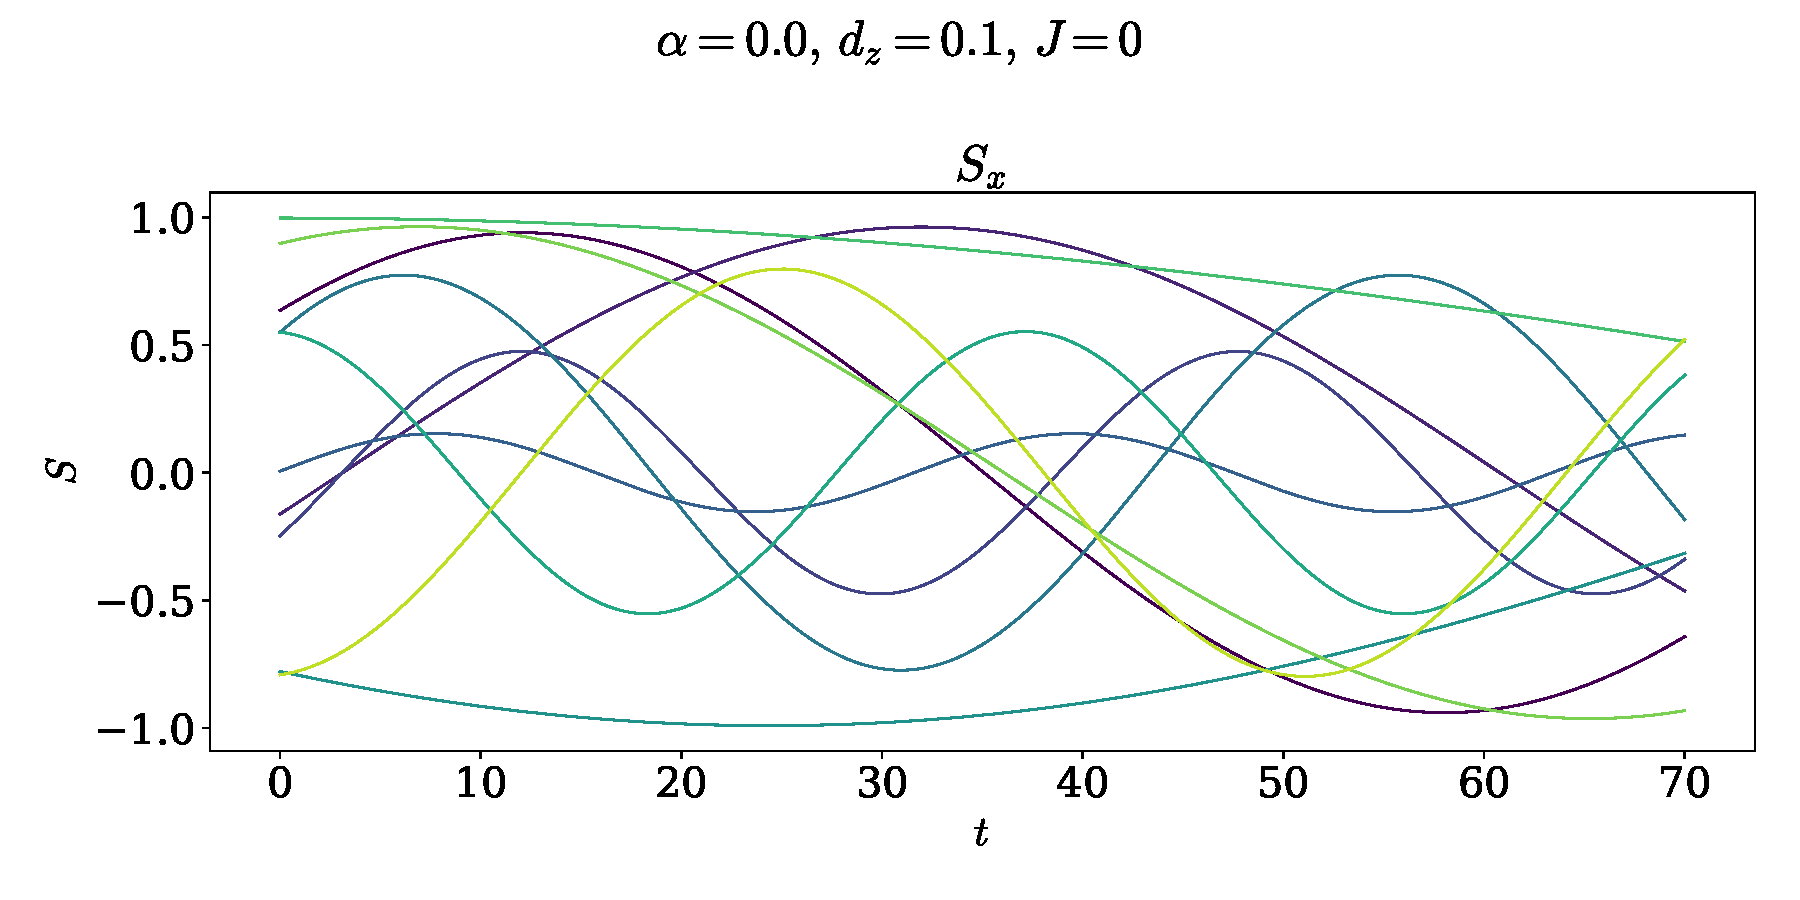
\includegraphics[width=0.8\textwidth]{../plots/2221a.pdf}
        \caption{The motion of the $x$-component of the spin of all spins in a chain, with anisotropy $d_z=0.1$. The frequency depends on $z$-component of the spin, which is why it varies.}
        \label{all tilted}
    \end{figure}


    \begin{figure}[H]
        \centering
        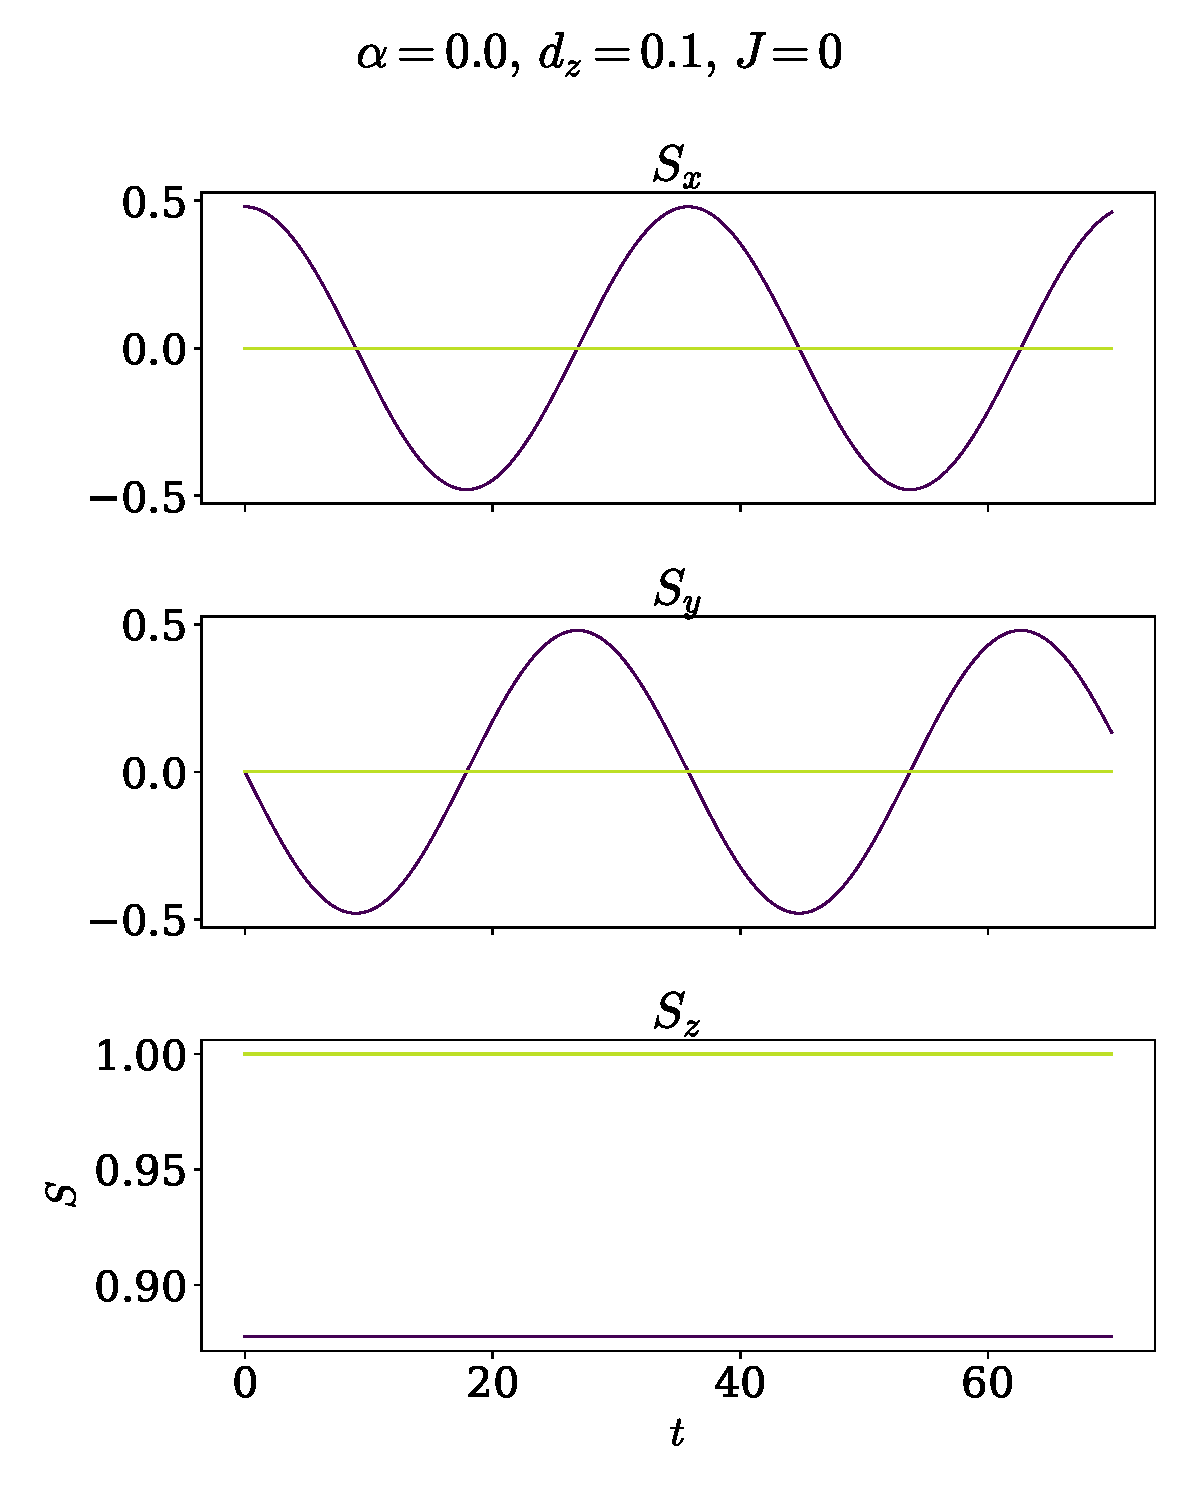
\includegraphics[width=0.49\textwidth]{../plots/2221b.pdf}
        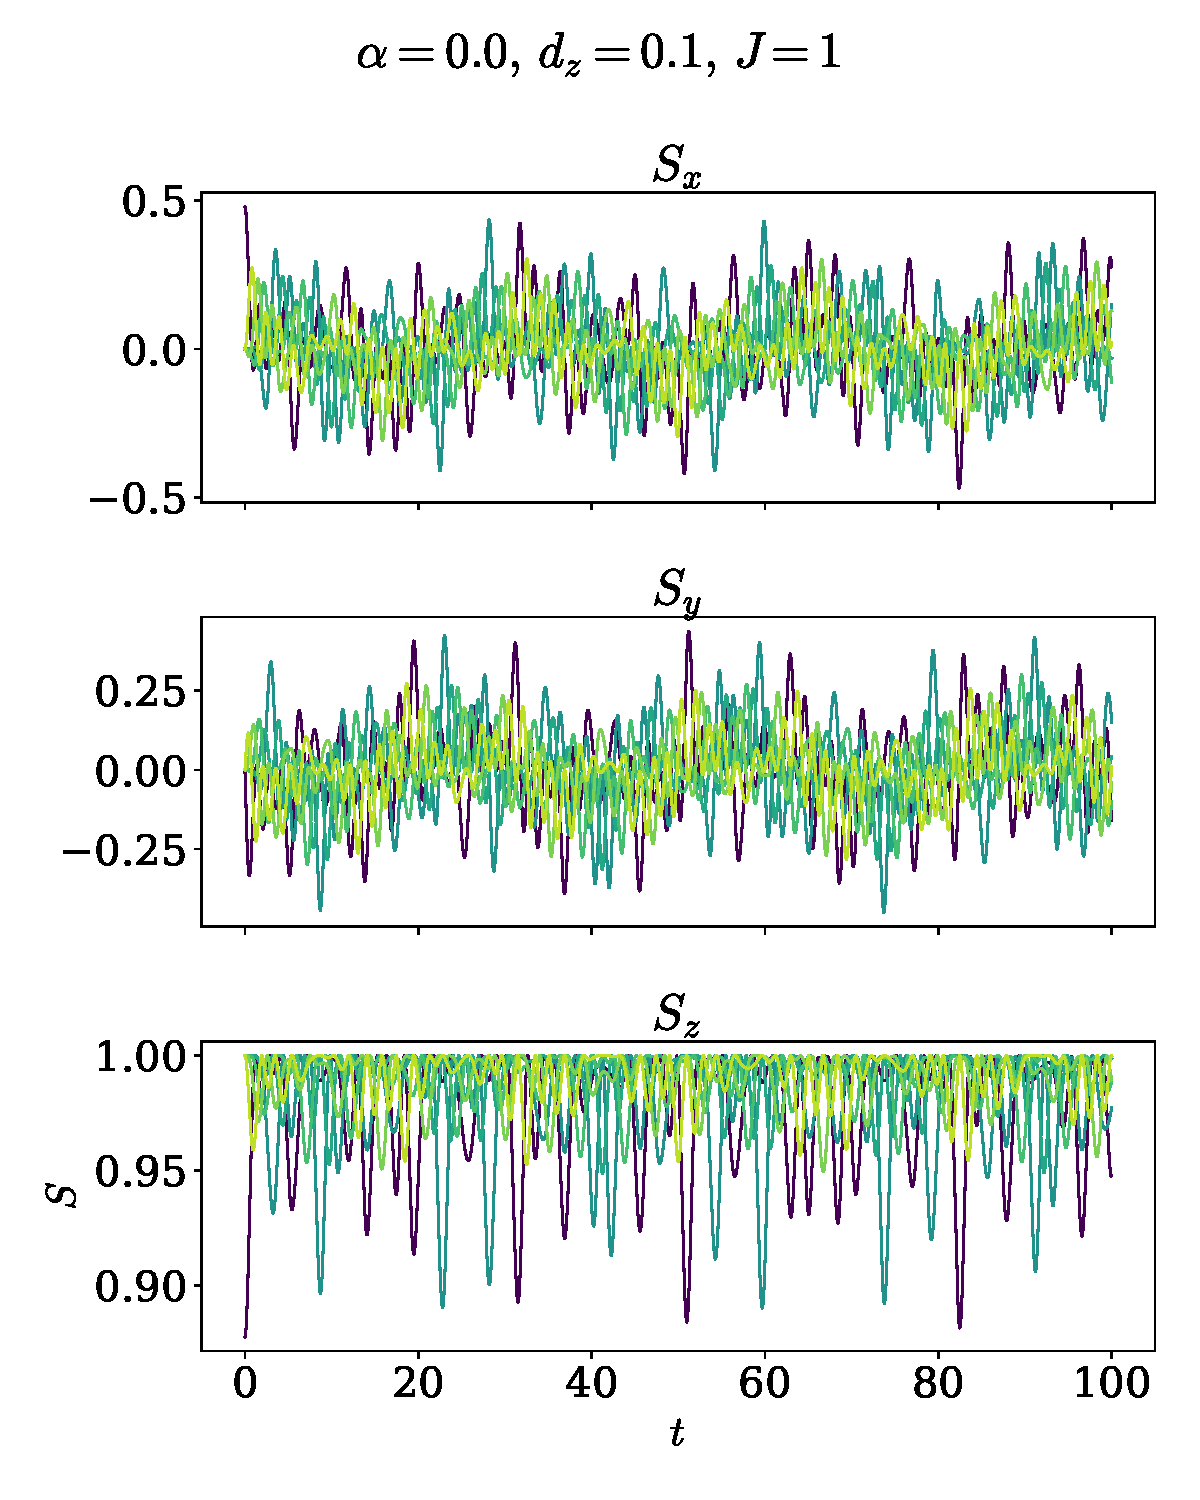
\includegraphics[width=0.49\textwidth]{../plots/2222.pdf}
        \caption{The motion of the different components of spin chains, with anisotropy $d_z=0.1$.}
        \label{one tilted}
    \end{figure}

    \begin{figure}[H]
        \centering
        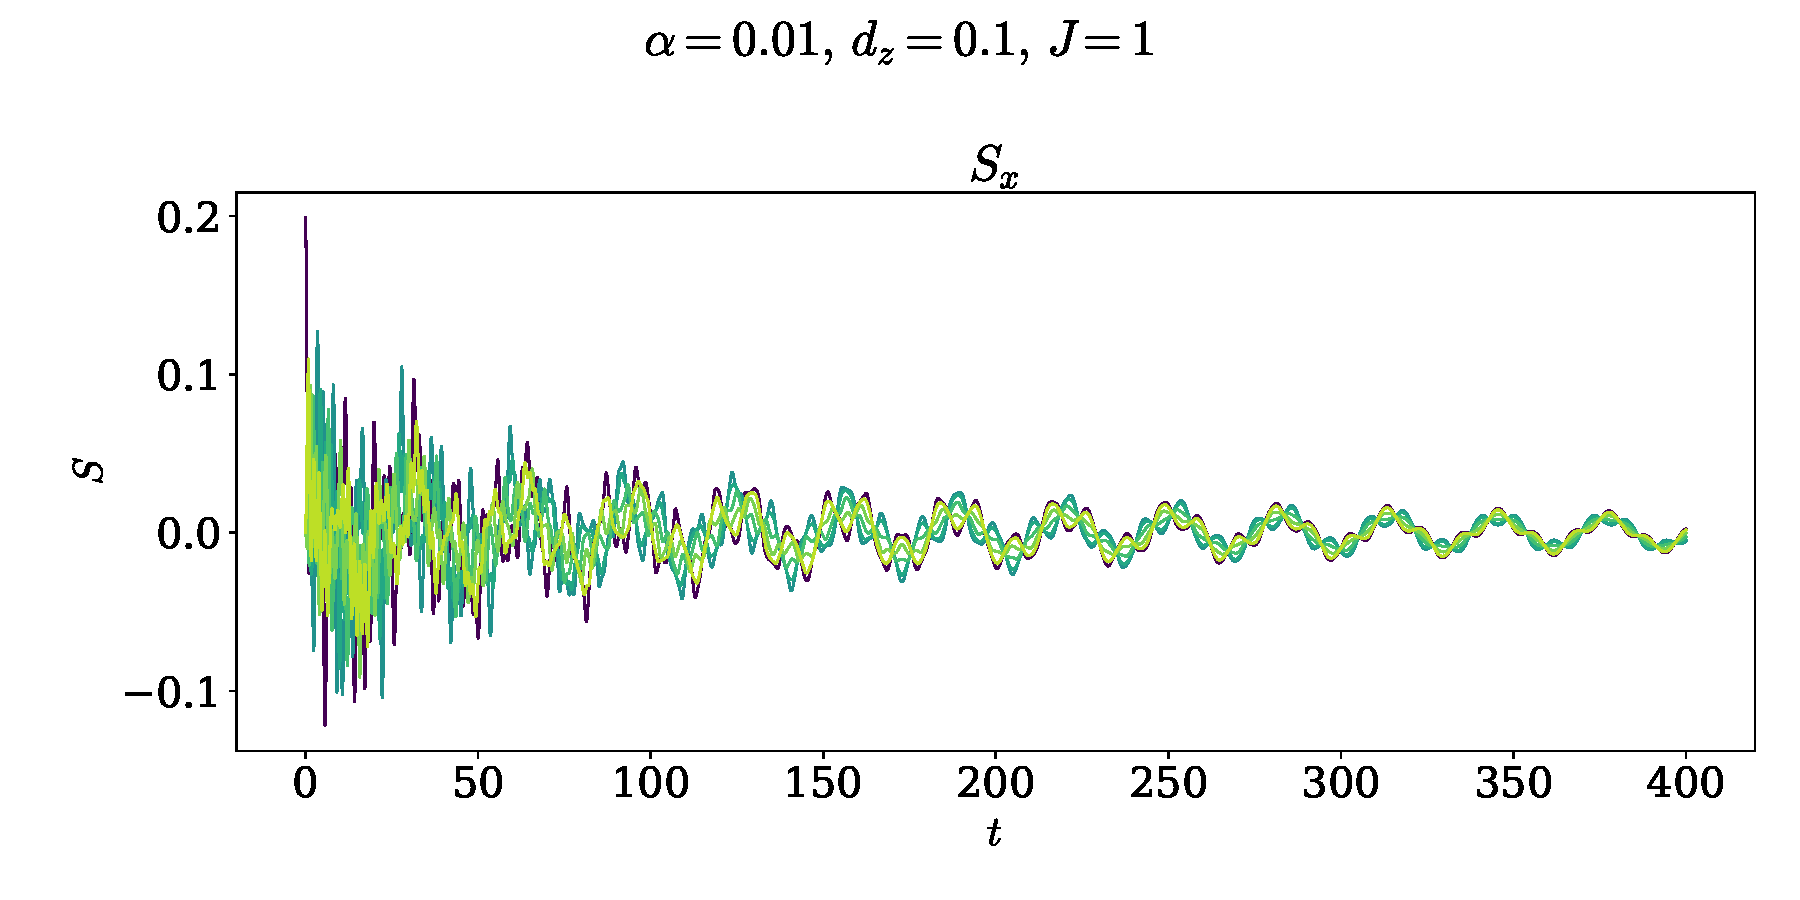
\includegraphics[width=0.55\textwidth]{../plots/2224.pdf}
        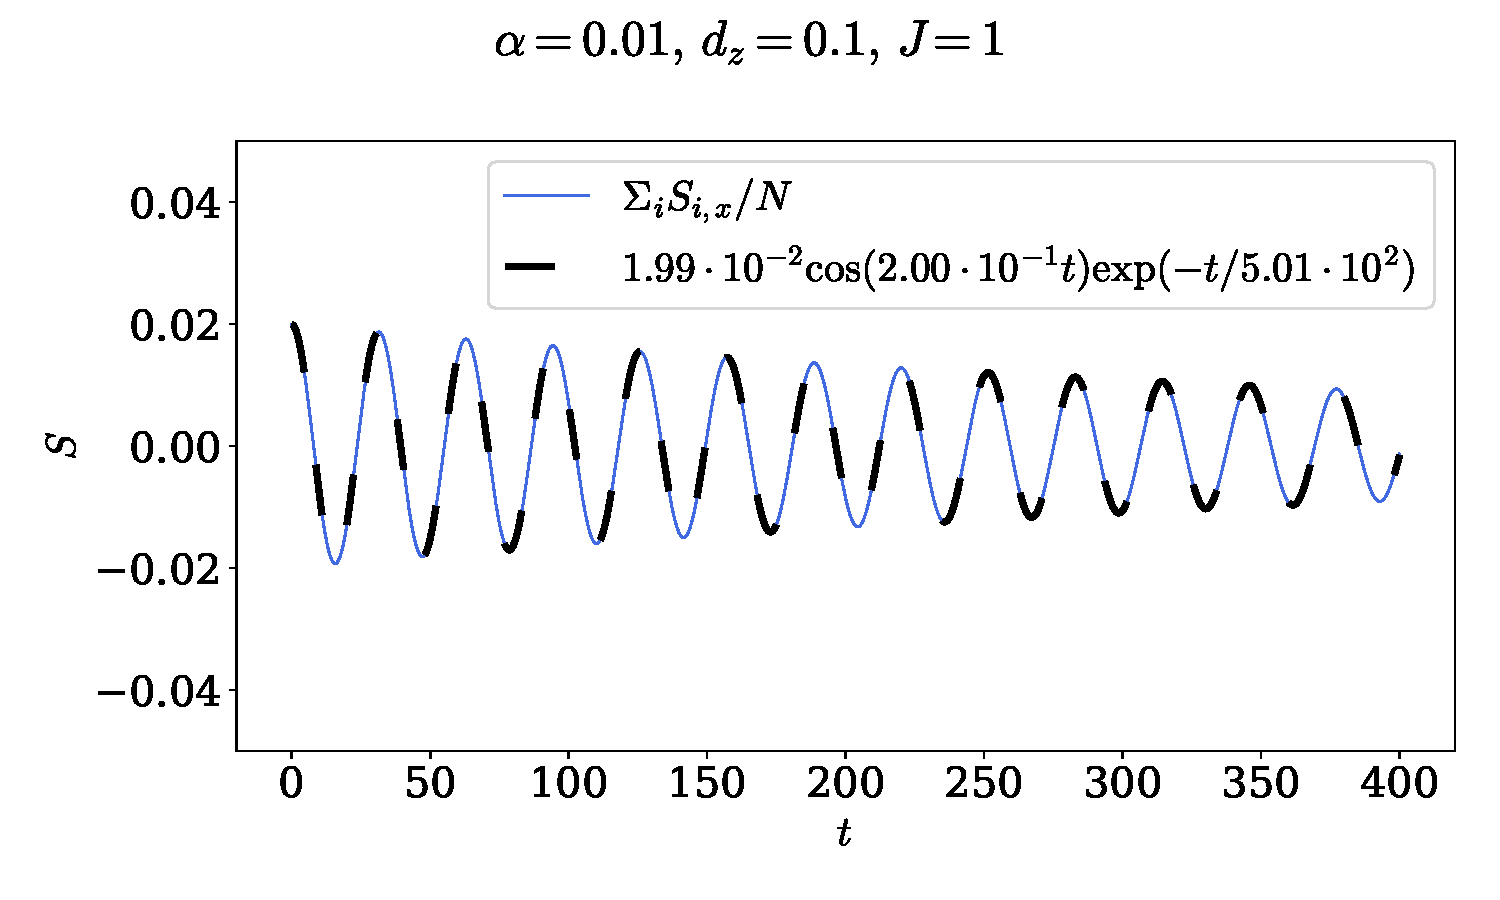
\includegraphics[width=0.44\textwidth]{../plots/2224fit.pdf}
        \caption{On the left, the $x$-coords all spins in a chain. On the right, the average of all the $x$-components, and a fitted function.}
        \label{one tilted dampend}
    \end{figure}


    \begin{figure}[H]
        \centering
        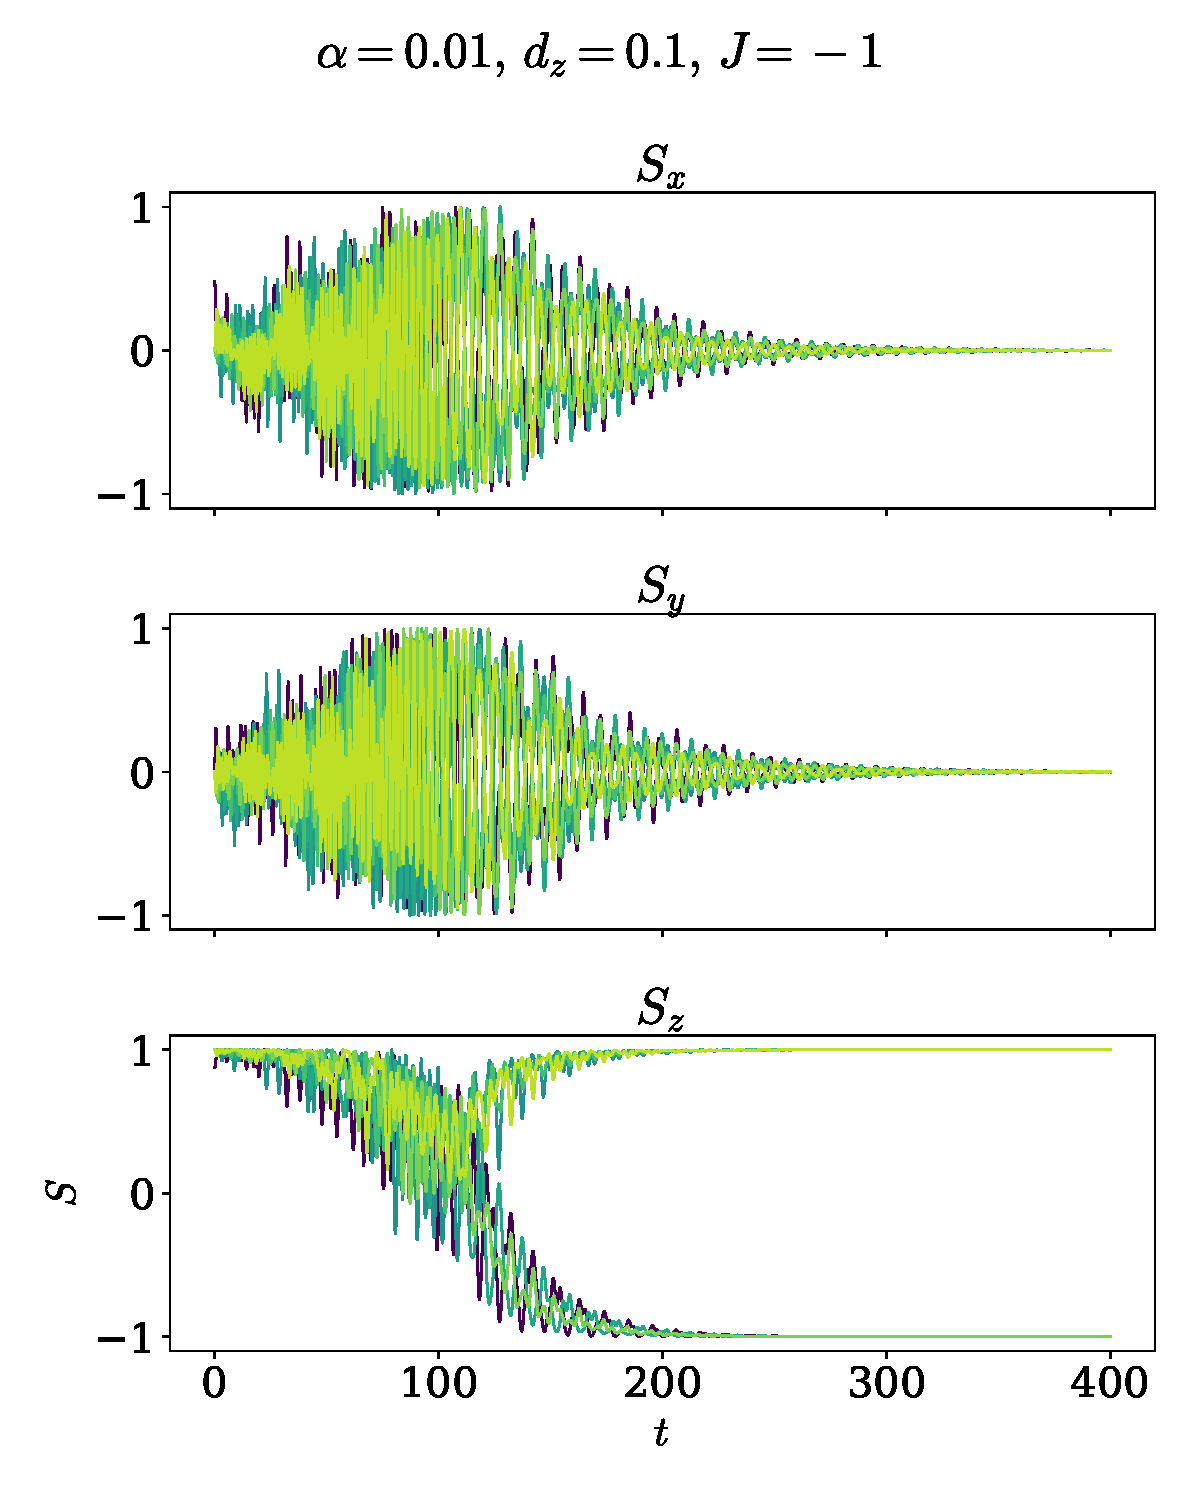
\includegraphics[width=0.49\textwidth]{../plots/2225.pdf}
        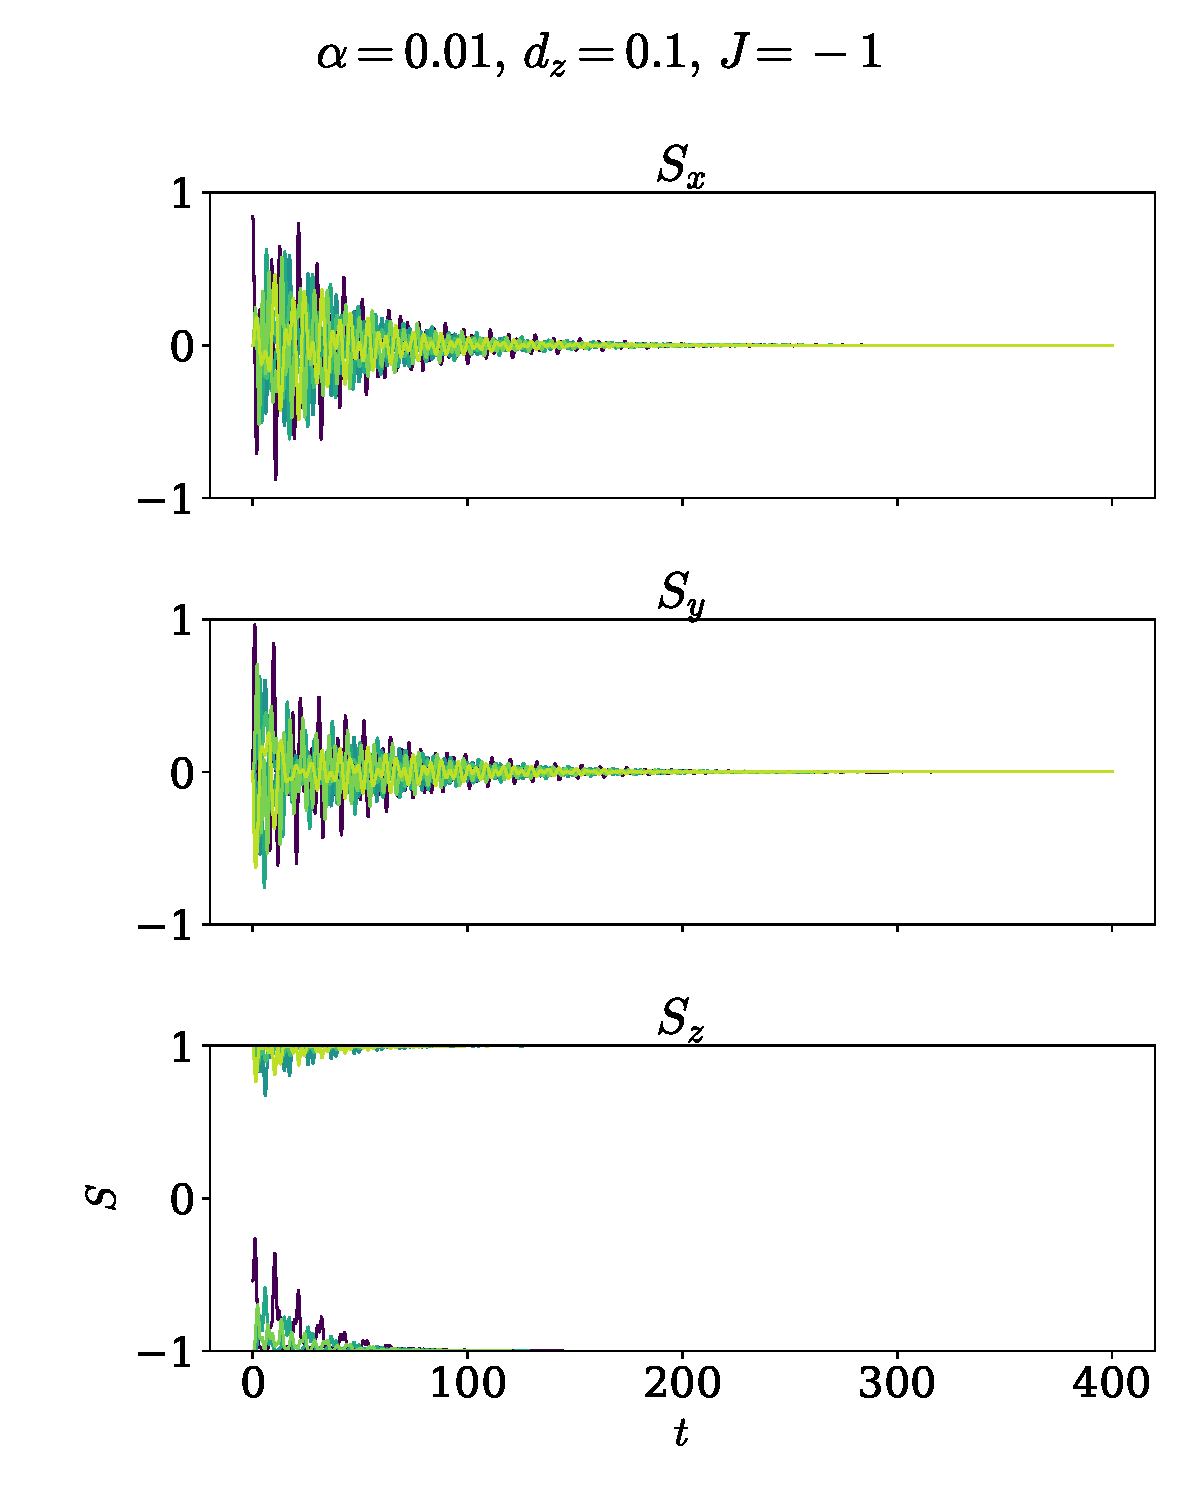
\includegraphics[width=0.49\textwidth]{../plots/22252.pdf}
        \caption{The components of the spins in an anti-ferromagnetic spin chain. The left starts with all spins almost aligned, the right almost in the groundstate for the anti-ferromagnet.}
        \label{one tilted dampend af}
    \end{figure}


    The magnetization of the state is, in the units previously described, given by
    \begin{equation*}
        M_a = \frac{1}{N} \sum_j S_{j, a}.
    \end{equation*}
    Thus, the magnetization of the ground state is in ferromagnetic case $\vec M = (0, 0, 1)$, while in the anti-ferromagnetic case $\vec M = (0, 0, 0)$.
    This means that a disturbance in the ground state of the ferromagnet, like the sustained magnon oscillation we showed earlier, will result in a sustained loss of magnetization.
    This is due to the fact that it is the state of maximum magnetization.
    This is showed in \autoref{mag}.
    Here, the magnetization quickly approaches the ground state value as the energy is dissipated.
    However, as the system settles in to the mode of sustained oscillation, the ferromagnetic on the left retains some loss in magnetization, while the anti-ferromagnet reaches the ground state much faster, and has no sustained difference in magnetization.


    \begin{figure}[H]
        \centering
        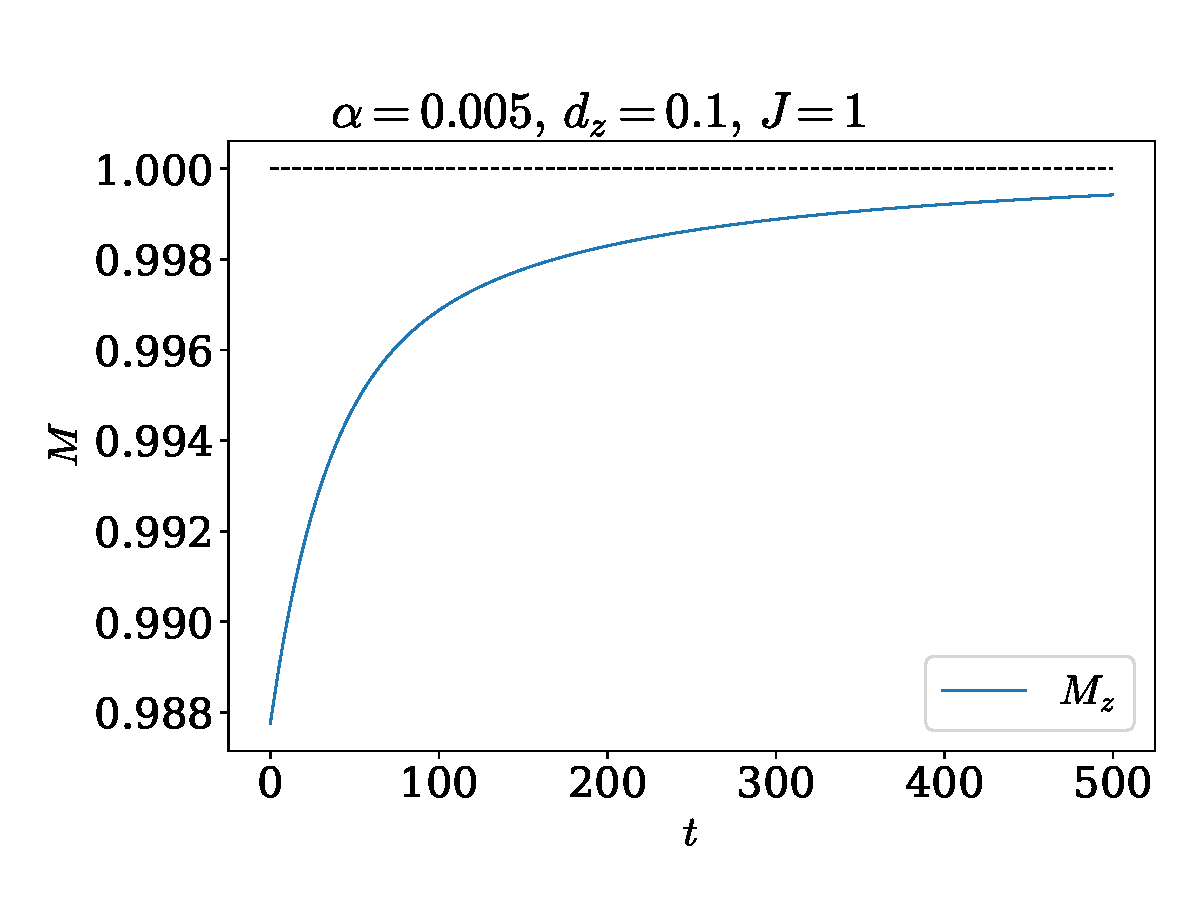
\includegraphics[width=0.49\textwidth]{../plots/mag.pdf}
        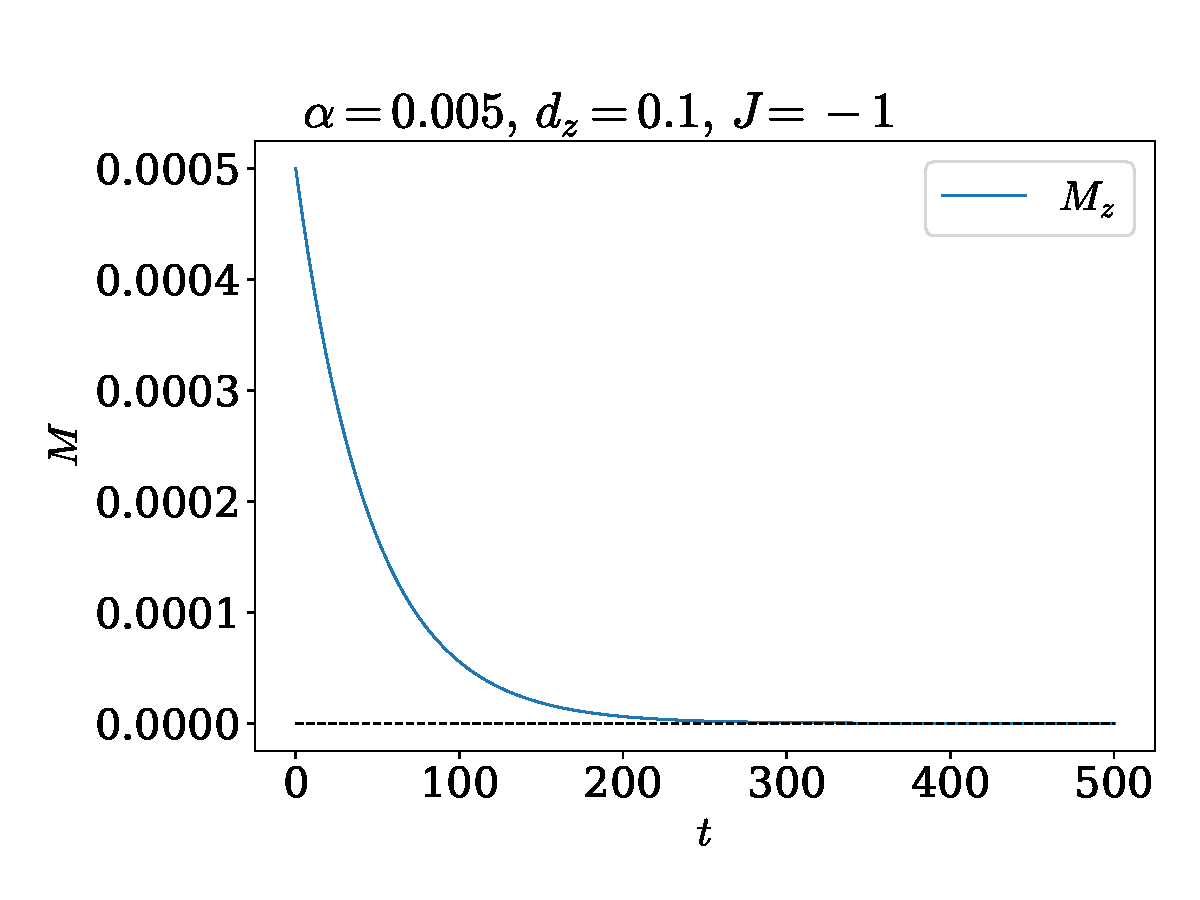
\includegraphics[width=0.49\textwidth]{../plots/mag2.pdf}
        \caption{The magnetization as a function of time, for a ferromagnet (right) and an anti-ferromagnet. Both systems are initiated with one spin slightly away from the ground state.}
        \label{mag}
    \end{figure}

    \section*{Conclusion}
    This report has documented the simulation of the classical Heisenberg model. By simulating a single spin, we have demonstrated that the expected that the analytical result is recreated, and the convergence properties of Heun's method.
    Ferromagnetic and antiferromagnetic states have different ground states, and anti-ferromagnetic reaches its ground state almost 10 times faster through dissipation than its ferromagnetic counterpart.
    Collective modes, magnons, is shown to exist in ferromagnetic materials.
    These modes are clearly visible in systems which are disturbed from the ground state, and has some dissipation.
    They affect the magnetization of the material, as they disturb it away from its highest magnetization state, the ground state.

    \printbibliography
\end{document}
